\documentclass{btswhitepaper}
\title{BitShares 2.0: Financial Smart Contract Platform}
\author{
 \IEEEauthorblockN{Fabian~Schuh}
 \IEEEauthorblockA{BitShares Europe, BitShares.eu\\
                   Erlangen, Germany\\
                   Email: \texttt{fabian@bitshares.eu}}
 \and
 \IEEEauthorblockN{Daniel~Larimer}
 \IEEEauthorblockA{Cryptonomex, Cryptonomex.com\\
                   Blacksburg (VA), USA\\
                   Email: \texttt{dan@cryptonomex.com}}%
 \thanks{This work was supported by Cryptonomex and honorable members of the
         bitsharestalk.org community.}
}


\begin{document}
\sloppy
\maketitle

\begin{abstract}%
 Ever since Satoshi Nakamoto released his whitepaper and corresponding software
 for bitcoin, the cryptocurrency ecosystem grew rapidly. Bitcoin created an
 ecosystem which everybody could use to \emph{transfer} value without
 unnecessary middlemen, banks or counterparty risk. Having the blockchain
 and consensus technology established and proven stable, the question arose
 whether this technology could be applied to allow \emph{trading} of multiple
 assets without the need for a broker or central entity.
 % Several so called bitcoin 2.0 projects (among which are BitShares 1.0, NXT,
 % Counterparty, Ethereum, \dots) showed the feasibility (DEX).
 The aim of BitShares 2.0 is to evolve the term \emph{decentralized exchange}
 (DEX) and not only provide trading of assets but also offer classical
 financial instruments on the blockchain. Two of these instruments --- market
 pegged assets and user-issued assets --- are discussed here.
 % With price stable digital tokens such as bitUSD, a whole new set of
 % financial contracts are now directly available through the decentral
 % exchange.

\end{abstract}
\section        { Introduction                                     } %%%%%%%%%%%%%%%%
% Smartcoins
%%%%%%%%%%%%%%%%
In todays world, crypto-currencies are unique in that they are the only digital
currency that is not someone else's liability. They are \emph{fungible},
\emph{decentralized}, and as \emph{valuable} as the network of users that
support them. Unfortunately, they suffer from very high volatility, because
their perception of value constantly changes as users enter and leave the
ecosystem. Although many professional traders appreciate this volatility, it
prevents its adoption as a \emph{payment} solution.

The traditional approach to creating a \emph{stable} asset is to accept
deposits and issue a digital token as a \emph{claim receipt} (i.e. ``I Owe
You''). Under this approach, the token is valued by the market as the
underlying asset, discounted by any credit risk associated with the issuer.
This can work well for transactions, but less well as a form of savings.
Furthermore, history has repeatedly proven that issuers eventually go bankrupt
due to fraud, incompetence, or government intervention.

%%%%%%%%%%%%%%%%
% MPA
%%%%%%%%%%%%%%%%
More recent alternative approaches have used a crypto-currency as
\emph{collateral} in a \emph{contract for difference} (CFD)~\cite{def:cfd}.
Under this approach, two parties take opposite sides of a trade, where one
party is guaranteed price stability, and the other party is granted leverage.
This approach works as long as sufficient collateral exists, and the contract
can be settled by an honest 3rd party with a price feed.

These contracts are \emph{derivative instruments} and part of a wider
definition of \emph{financial instruments}. Since financial instruments is
defined as \emph{tradable} assets of \emph{any} kind they can (in general) be
cash, proof of ownership, or a contractual right to receive or deliver a
financial instrument. 

BitShares, as a decentral counterparty-trust-free platform for financial smart
contracts which operates over the internet, offers a set of financial
instruments including CFDs. Several other financial instruments are fully
implemented, one of which can act as \emph{derivative} with \emph{cash} as
underlying asset. These derivatives contracts derive its value from the
performance of an underlying entity and are thus often referred to as
\emph{market pegged assets} (MPA) or ``smart-coins'', and will be presented in
\cref{sec:mpa}.

%%%%%%%%%%%%%%%%
% UIA
%%%%%%%%%%%%%%%%
Additionally, the BitShares platform provides an abstract feature known as
"user-issued assets" (UIA) to help facilitate as wide range of profitable
business models for certain types of services. The term refers to a type of
custom token registered on the platform, which users can hold and trade within
certain restrictions. The creator of such an asset publicly names, describes,
and distributes its tokens, and can specify customized requirements, such as an
approved \emph{whitelist} of accounts permitted to hold the tokens, or the
associated trading and transfer fees. These tokens allow for diverse use-cases
such as, for instance, ownership tracking, crowd fund raising, IOUs, coupons,
and many more and will be discussed in \cref{sec:uia}

%%%%%%%%%%%%%%%%
% DEX
%%%%%%%%%%%%%%%%
In order to \emph{trade} financial instruments, BitShares provides a
high-performance \emph{decentral exchange} (DEX), with all the features expect
from a trading platform (see \cref{sec:dex}). Any two assets that are
registered on the blockchain (MPA or UIA) may be traded against each other at
any time. Orders can be settled almost instantly up to at least 100.000
transactions per second.  With this kind of performance on a decentralized
exchange, there is no more need to risk funds in centralized exchanges.

% %%%%%%%%%%%%%%%%
% % Bonds
% %%%%%%%%%%%%%%%%
% Last but not least, the BitShares bond market (currently not implemented fully)
% is an investment marketplace accessible to anyone that lets you earn interest
% with any of your asset, or take a short position using any other asset as
% collateral.

In the following we will discuss the financial instruments available in the
BitShares network as well as the DEX. It is recommended to previously read
through the basic technological components of BitShares in the other white
papers~\cite{bts:general,bts:growth,bts:structure}.
 

\section        { Market Pegged Assets (MPA)                       } BitShares' market pegged assets (MPA), or \emph{Smartcoin} (as they is often also
called) are a new type of freely traded digital asset whose value is meant to
track the value of a conventional asset such as the U.S. dollar or 1 ounce
of gold. What makes market pegged assets unique is that they are free from
counter party risk.

A currency with the properties and advantages of Bitcoin that maintains price
parity with a globally adopted currency such as the US dollar has high utility
for convenient and censorship resistant commerce. A SmartCoin (synonym for
Market Pegged Asset) is a cryptocurrency that always has 100\% or more of
their value backed by the BitShares core currency, BTS, to which they can be
converted at any time at an exchange rate set by a trustworthy price
feed\footnote{Price feeds are published by delegates that have shareholder
approval.}. 
 
This paper will explain how market pegged assets including (for instance)
\emph{BitUSD} (intended to track the value of the US dollar) achieve price
parity while minimizing risk to holders.
 
\subsection     { Price Stability                                  } Ever since the bitcoin blockchain initiated the age of decentral public
ledgers, economists and engineers are trying to achieve a stable cryptocurrency
or a price pegged crypto token. The following two subsection want to discuss
the meaning of a ``stable'' currency and show how BitShares want's to fill the
gap.
 
\subsubsection  { Definition of Price Stability                    } Before we discuss how BitShares achieves price \emph{stability} we first need to
define what properties make a currency \emph{stable}.

In the U.S., for instance, the Federal Reserve (FED) has a mandate of
\emph{stable prices} and it is almost universally accepted that this is a good
mandate. The same holds true for the Euro with its stability being
\emph{controlled} by the European Central Bank (ECB). Mostly every
country/nation or federation applies a similar concept.

However, it is also widely accepted among many crypto-currency fans that, in
the case of the US dollar, the FED has failed at their mandate because of
monetary inflation and increase in the money supply. Since monetary inflation
is a sustained increase in the general level of prices, it is equivalent to a
decline in purchasing power of money. Hence, a dollar buys less and less over
time. As a result, we see the dollar losing 99\% of its \emph{purchasing power}
since the FED was founded in 1913~(see \cref{fig:monetarybase}). 

\begin{figure}[!htp]
 \centering
 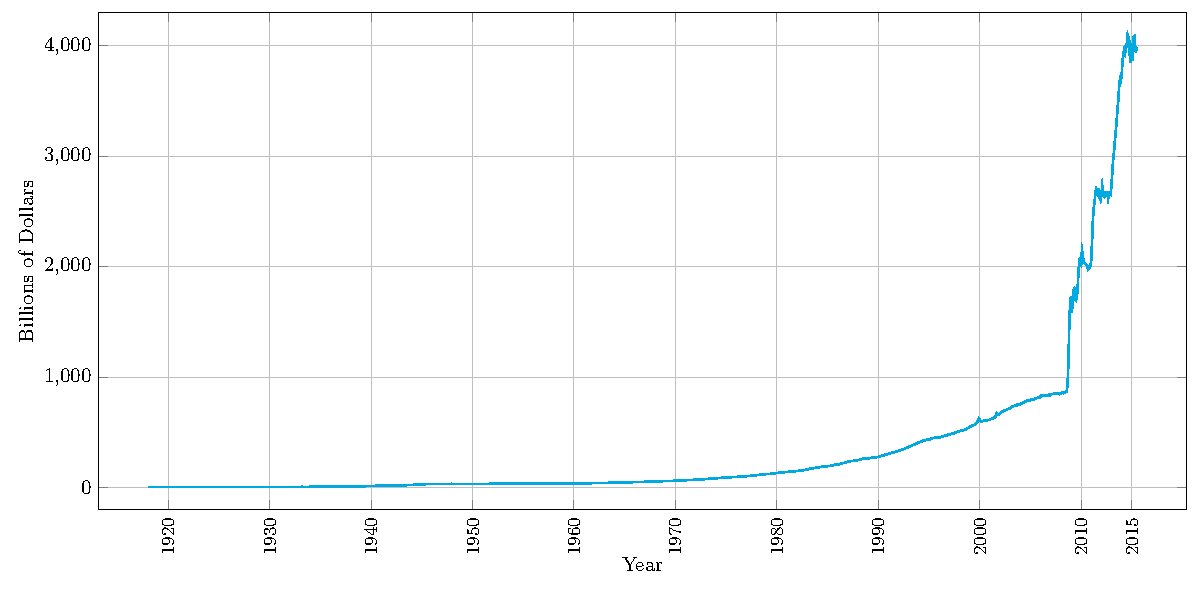
\includegraphics[width=\linewidth]{figures/monetary-base}
 \caption{St. Louis Adjusted Monetary Base~\cite{ambsl}}
 \label{fig:monetarybase}
\end{figure}

The goal of this paper is not to propose a replacement of central banks but to
clarify the terminology in particular with regards to ``stable''
cryptocurrencies. Unfortunately, some people in the cryptocurrency space are
attempting to provide an alternative currency that can achieve the same
mandate. However, since price stability at its heart is the same as \emph{price
fixing}, this is a well known economic fallacy that crypto-currencies should
avoid.

% The goal of the FED price stability mandate is to mask the systematic theft of
% all increases in the production efficiency of the economy. 

Imagine a central bank managed to keep prices stable through their monetary
policy with 0\% price inflation over 20 years. Now lets assume that during this
same 20 years the advances in robotics and automation resulted in a 3x increase
in efficiency and thus there are now 3x as much food, cars, phones, houses,
etc. For the sake of this example we will assume the population is the same and
everyone has the same amount of money in the bank. You would normally expect
that everything would be 1/3 the price and that everyone would be able to
afford 3x their prior life style. But because of the central bank's
intervention they have managed to also increase the money supply by 3x.
% and distribute it in secret. The end result is that some people get a 1000x
% increase in life style while everyone else stands still.

% FIXME: not very neutral!
% We can conclude from this example that the mandate for price stability is
% mostly a goal meant to mislead the general public and mask theft from the lower
% and middle classes on a massive scale even at 0\% price inflation. For this
% reason, we do not want to bring this same mandate to crypto currencies but
% instead aim to free us from monetary enslavement.

We notice that the goals should not be \emph{price stability} nor should we
target a \emph{stable value} or \emph{purchasing power} (at least not yet). 
%
What we want to achieve instead is 
\begin{itemize}
 \item a \emph{predictable} price with \emph{reduced volatility}
 \item a somewhat reliable ability to \emph{predict the future value} of a token, and
 \item a unit of account that doesn't have any meaningful capital gains or
       losses for tax purposes.
\end{itemize}

Hence, price ``stability'' really means price \emph{predictability} within some
tolerance level. In the case of the U.S. dollar, a willingness to accept a 5\%
loss (in purchasing power) per year via deflation, demonstrates that
predictability is more important than stability~\cite{bm:stable:impossible}.
 
\subsubsection  { BitAssets 1.0: Historical Lessons                } \label{sec:bitassets1}

The first proposal of the BitAsset system has evolved over 9 months since it
first launched as we learned how market participants reacted to various rules.
We notices that, liquidity is critical to confidence in the value of the token
and that a system with unbalanced rules will tend to bias the price in one
direction or the other.

Early on, BitUSD was driven down to \$0.85 as demand for shorting outstripped
demand for BitUSD and shorts were not forced to cover. Then, after implementing
a \emph{30 day forced covering rules}, the price stabilized around \$0.98 to
\$1.00. Later, as the cryptocurrency bear market progressed, we had BitUSD
trading at \$1.05 or more because everyone is scared to use leverage and those
that have open positions looked to cover their position while those who held
BitUSD were not looking to sell. Over the course of these past 9 months, we
have seen 3 different markets and had an opportunity to better understand the
behavior of market participants and improve the protocol accordingly.

We have seen that the idea of a market pegged crypto token can in general work,
but obviously, we were not satisfied as to \emph{how well} BitAssets 1.0
worked. For that reason, the improved BitAssets 2.0 protocol was proposed which
will be described in the following.
 
\subsubsection  { BitAssets 2.0: Evolving a Stable Crypto Currency } For BitUSD to be accepted as being equal to \$1.00 for the purposes of setting
prices, it only needs to maintain a \emph{floor} of \$1.00. If it can maintain
a floor of \$1.00, then merchants can accept it and know their margins are safe
and that they are \emph{not exposed to currency risk}. In order to enable a
guaranteed floor, all BitUSD can be \emph{force liquidated} at a trustworthy
price feed\footnote{Price feeds are published by \emph{witnesses} that have
shareholder approval. See~\cref{sec:feeds}.}. Since this rule is present,
those who create the BitUSD must sell it at a price that properly accounts for
this risk of \emph{forced settlement}. This means that at almost all times, new
BitUSD will only enter circulation when there is a buyer willing to pay a
premium for a guaranteed floor.

As we will see, since USD holders can initiate settlement, there is no need for
artificial forced covering every 30 days. This relieves shorts of risk, helps
increase short demand, and keeps the price of BitUSD near the floor.
 
\subsection     { Price Feeds                                      } \label{sec:feeds}

The blockchain needs to be aware of the external price of BTS in order for
settlements to convert SmartCoins into the core asset (BTS) at a fair price.

In BitShares, this is achieved by means of a set of $N$ trusted
\emph{witnesses}. These witnesses have to be elected by the corresponding
BitShares shareholders (e.g. holders of BTS) and can be constantly reviewed as
all prices are put on the blockchain in a public manner by means of
transactions of a certain type. Hence, misbehaving witnesses can be identified,
``fired'' and lose their reputation of shareholders.

Additionally, to prevent manipulation of the price feed, $N$ witnesses have to
be elected that can all produce their prices independently. Having a set of $N$
prices $p_i,\;1<i<N$ for an arbitrary MPA on the blockchain, the protocol
obtains a single price $\tilde{p}$ by the use of the \emph{median} according
to:
\begin{align}
 x &= \operatorname{sort}(p[i])\\
 \tilde p &=\begin{cases}
   x[\frac{N+1}{2}]                                               & N \text{ odd}\\
   \frac {1}{2}\left(x[{\frac{N}{2}}] + x[\frac{N}{2} + 1]\right) & N \text{ even.}
 \end{cases}
\end{align}
Hence, the price is resistant against misbehaving witnesses in that only a
majority of price publishers can manipulate the outcome of the median. In
practice, any unintentional feed \emph{error} is thus balanced around the true
price. % FIXME later, show some statistics from bts-0.9

Obviously, the shareholders are required to constantly monitor the published
prices of their witnesses and should make a public note about any
discrepancies. This is similar to traditional \emph{quality management} for the
\emph{Smart Coin} products (e.g. bitUSD) and BitShares system can offer a paid
position to perform this service.
 
\subsubsection  { Price Manipulation                               } There is always concern of price manipulation. Someone with a large amount of
money on both sides of a trade can use their funds to manipulate the markets
and thus the price feed. If the amount of money they lose manipulating the
markets is less than the amount of money they can gain by manipulating the
price feed, then it will be profitable to manipulate the market at the expense
of either the BitUSD longs or the shorts. A low-collateralized short that sees
a large force-settlement order requested can attempt to manipulate the markets
and thus the feed against the BitUSD holder.

The risk of price manipulation is priced into the premium on BitUSD charged by
the shorts, and thus should already be priced into the market. If price
manipulation became a serious problem that caused very high premiums, then it
could be addressed by the price feed producers, who can adopt a moving average
over wider time windows to increase the difficulty of short-term manipulation.
A variety of algorithms could be used to estimate a ``fair price'' that keeps
BitUSD valued at least \$1.00.

In practice, a feed producer can observe the BitUSD-to-USD market as an
indicator on which way to adjust the feed. Generally speaking, the strategy
that the feed producers adopt for controlling the feed should be public
knowledge, because the shorts will ultimately rely on it. For the feed
producers to change strategies in unpredictable ways could cause losses to both
longs and shorts.
 
\subsection     { Issuance and Supply of Collateralized Smartcoins } \label{sec:mpa:create}

A BitShares MPA can be viewed as a contract between an asset buyer seeking
price \emph{stability} and a short seller seeking greater \emph{exposure} to
BTS price movement. The open source BitShares software protocol implements a
decentralized marketplace for MPA where all transactions are recorded on the
shared block chain ledger and the software enforces the market rules. This
block chain based marketplace is referred to as the \emph{decentralized
exchange} or \emph{internal market} (c.f., \cref{sec:dex}) to distinguish from
\emph{external markets} such as websites that facilitate the exchange of
government issued currencies with cryptocurrency.

SmartCoins are tokens of a particular MPA (e.g. bitUSD). They use the concept
of a contract for difference, and make the long side fungible. For the purpose
of this discussion, we will assume that the long side of the contract is BitUSD
and that the backing \emph{collateral} is BTS (the BitShares core asset).

In practice, bitUSD are created on the BitShares blockchain when a BTS holder
asks the network for them by handing over \emph{collateral} to the network,
essentially locking them in a contract for difference (c.f., \emph{1)} in
\cref{fig:btsdex}).

\begin{figure}[!htp]
 \begin{center}
  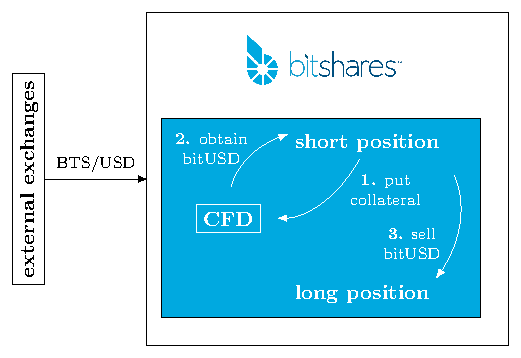
\includegraphics[width=.8\linewidth]{figures/external-pricefeed}
 \end{center}
 \caption{Illustration of external price discovery and a ``short sell'' to seek
          greater exposure for BTS price movements.}
 \label{fig:btsdex}
\end{figure}

The collateral is only returned to the short seller when the corresponding
amount of the asset agreed in the contract is handed over to the BitShares
network again. The protocol will then effectively destroy these tokens and
fulfill the contract. This is referred to as \emph{covering a
short}. At the moment of creation, the position of the \emph{shorter} has not
changed at all because he can directly cover his own short position using the
bitUSD to gain back his BTS used as collateral.

If the short seller has sold the SmartCoins he has created, then he would be
required to purchase them back from the market before closing his short
position. Meanwhile, if the value of the collateral relative to the current price
of the market pegged asset falls below a certain margin of safety, the assets
can be automatically (i.e. initiated by the protocol itself) repurchased from
the market before the collateral becomes insufficient.

These rules create systemic demand for market pegged assets while allowing them
to remain fungible. To protect your contract against \emph{margin calls}
(automated, network initiated force settlement of your contract at the price
feed), you should at least maintain the so called \emph{maintenance collateral
level} at all times. Hence, the collateral only needs to be high enough to
cover any slippage as a result of a short squeeze.

In summary, the following set of market rules apply to all market pegged assets
(for the sake of simplicity, we here focus on the MPA bitUSD):
\begin{itemize}
 \item Anyone with BitUSD can settle their position within an
       interval\footnote{defined by the shareholder approval} at the settlement
       price (identical to the feed price).
 \item In this case, the \emph{least} collateralized short positions would be
       margin called and their collateral would be used to settle the position.
 \item The price feed is the median of many sources that are updated at least
       once per hour.
 \item Short positions never expire, except by hitting the maintenance
       collateral limit, or being force-settled as the least collateralized at the
       time of forced settlement (see point 2).
 \item In the event that the least-collateralized short position lacks enough
       collateral to cover at the price feed, then all BitUSD positions are
       automatically force settled at the price of the least collateralized
       short (black swan event, see~\cref{sec:blackswan}).
\end{itemize}

These simple rules enable a price floor of \$1.00 for 1.00 BitUSD. A simple
metric for testing the validity of our claim is to demonstrate that, if you can
find someone willing to sell 1.00 BitUSD for \$1.00, that it would be the
cheapest option for buying BTS. This means that 100\% of the buying demand for
BTS would be available to give liquidity to BitUSD holders as a priority over
BTS holders.
 
\subsection     { Perspectives of Participants                     } While the rules are simple, the consequences are less obvious. Let's analyze
this from the perspective of the various players.
 
\subsubsection  { The Short Position                               } When deciding a price at which to enter a short order, a trader must consider
the risk of forced settlement. In this case, no trader will attempt to short at
or below the price feed, because they could be forced to settle at the price
feed. In fact, a smart trader would allow enough of a spread to account for the
risk of being forced to settle at a feed price that was off by a small amount.
In practice, the risk posed by the feed error is balanced equally between being
in the favor of the short and in the favor of the long, leaving only the risk
of being forced out of their position at an inopportune time.

A short can minimize their exposure to the feed by providing enough collateral
to keep far above the least collateralized positions, and thus very unlikely to
be forced to settle at the feed or at an inopportune time.

In practice, the only way new BitUSD enters circulation is if there is someone
willing to pay enough of a premium to convince a short to provide guaranteed
liquidity at the price feed on demand, while also covering the cost of exchange
rate risk. This premium will be higher for the backing cryptocurrency in a bear
market, and will be lower in a bull market.

Someone who is short has only one way to exit their position: by buying BitUSD
off the market. This means that a short must also factor in the risk that the
premium may change. If a short position is entered in a bull market with a 0.1%
premium, it may be forced to exit during a bear market with a 5% premium. In
this event a short position is exposed to both exchange rate of the dollar vs.
BTS and the premium risk. On the other hand, a short entered during a bear
market with a 5\% premium may get to cover during a bull market with a .1%
premium.

For all intents and purposes, the premium is expected to move in the same
direction as the price, and thus speculators who only care about relative price
changes can ignore the premium.
 
\subsubsection  { The Long Position                                } The very first buyer of BitUSD will have to pay the lowest premium set by the
shorters. For the sake of discussion, let's assume the first BitUSD was created
in a bear market and cost \$1.05 to create. The holder of that BitUSD has two
options: sell it on the market for \$1.04, or request forced settlement for
\$1.00. Clearly, the forced settlement option would only be used in situations
where there was a decrease in total demand for BitUSD and there were no offers
to buy it above \$1.00.

As a trader only looking to trade back and forth between BitUSD and BTS, this
premium doesn't matter. Such as trader is exposed to volatility in the premium,
but that risk is limited to \$0.05 in this example. In practice, the premium is
expected to be relatively stable and predictable.
 
\subsubsection  { The Customer's Perspective                       } Customers use BitUSD because it provides them the convenience and freedom of a
crypto-currency, and has lower transfer fees compared to most other payment
platforms besides being significantly more convenient than fiat.

A customer looking to buy goods and services with BitUSD finds himself paying a
premium to acquire BitUSD from the market. This means that customers will
prefer merchants that offer a discount equal to the premium paid. On the other
hand, the premium is a wash for a customer that \emph{earned} BitUSD at a
nominal value of \$1.00.

In fact, the only people to whom the premium matters are those who are looking
to \emph{enter} or \emph{exit} the ecosystem. Once a customer or merchant is
within the ecosystem, it is easy to simply trade BitUSD at parity, even if it
is theoretically worth slightly more outside the ecosystem.

Of course, merchants and customers are free to negotiate the best way to split
the premium, and the free market will take care of the rest. In the mean time,
all participants can rest assured that BitUSD is always worth \emph{at least}
\$1, and can consider the premium for entering the ecosystem as a one-time fee
comparable to fees required for the exchange of foreign currencies.
 
\subsubsection  { The Merchant's Perspective                       } A merchant wants to be able to price merchandise in BitUSD, and obtain real USD
in the bank account, in a reasonable time, with minimal risk. In this case, a
merchant would place BitUSD on the market at \$1 per BitUSD. As discussed, BTS
buyers are looking for the opportunity to buy BitUSD at that price.

A smart merchant might recognize that 1 BitUSD can actually fetch \$1 plus a
variable premium, and start preferring that customers pay them in BitUSD at
face value. An even smarter merchant might offer a discount to customers that
pay in BitUSD.
%FIXME : is it wise to use smart/smarter in a whitepaper?

In any case, merchants have a financial incentive to advertise BitUSD as the
preferred payment mechanism, because they know that \$1.00 is the lower bound
on what BitUSD is worth.
 
\subsubsection  { BTS Shareholders and Investors                   } A buyer with dollars, looking to buy BTS, knows that 1 BitUSD can be used to
buy \$1 worth of BTS (plus the current premium). He also knows that this premium
can never be negative, because of the option to force-settle at the price feed.
In this situation, he can know with certainty that if he can convince someone
with BitUSD to sell for \$1.00, he can buy more BTS than if he simply buys BTS
with his dollars directly. The higher the premium, the more incentive exists to
buy BitUSD for \$1.00.

This means that, in a BTS bear market, the BitUSD price gives the highest
premium of the BTS price, and BitUSD becomes the easiest to sell. In practice,
the BitUSD:USD market will reflect the premium, and traders will usually be
unable to find anyone willing to sell for exactly \$1.00.

If a buyer is looking to purchase a large quantity of BTS without moving the
price, he can start by buying up BitUSD with dollars. This will slowly raise
the BitUSD:USD price, which is a signal to other market participants. A careful
buyer might be able to avoid signaling the market. Then, after acquiring the
position in BitUSD, the buyer can request a global settlement and get the price
feed on the entire purchase.

Because all positions and trades are visible on the blockchain, all of this
trading activity can be factored into the price, minimizing any potential
profits to be made by attempted manipulation.
 
\subsection     { Undercollateralization and Black Swans Events    } All guarantees of SmartCoins are subject to the caveat that a SmartCoin can
never be worth more than the collateral backing the least-collateralized short
position. In normal market conditions, the value of the collateral is always
more than sufficient, but, from time to time, markets can rapidly revalue the
collateral. If this revaluation happens faster than the short positions can be
forced to cover, then all SmartCoins are liquidated at the exchange rate of the
least collateralized short position. This is similar to an insolvent bank
converting its deposits to equity.
 
\subsection     { Risks                                            } The current implementation of market pegged assets in the BitShares system is
designed to minimize risk of loss to market pegged asset holders. Short
positions are opened with collateral worth three times the market value of the
asset. The initial collateral is comprised of the BTS paid by the buyer for the
asset and twice this amount of BTS contributed by the short seller. The
collateral requirements and margin triggers were chosen conservatively to
protect the holders of market pegged assets from volatility of the underlying
collateral. Forcing short positions to cover every 30 days provides additional
assurance of short term liquidity. Control over the price feed is distributed
among over 50 separately elected delegates who compile information from
multiple exchange sources. Despite such precautions, it is important to
carefully explore risks of using the system. Risks can be broadly categorized
as value risk, counterparty risk, or systemic risk.
 
\subsubsection  { Collateral Risk                                  } Market pegged assets maintain their price parity due to being backed by
collateral that has an established real world value. When the value of the
collateral falls, the system is designed to react by driving the internal asset
exchange to match the new real world exchange rate and trigger \emph{force
settlements} (also known as margin calls) if necessary.

% First half of the paragraph contains dublicated information from
% fp-mpa-blackswan.tex
However, there exists a possibility that the underlying collateral (BTS) drops
in value so quickly the market pegged assets become under-collateralized. Often
termed a \emph{black swan event} (c.f., \cref{sec:blackswan}), a sudden crash
of BTS value could prevent the system from adjusting in time. In this event,
the full amount of collateral is no longer sufficient to purchase the market
pegged asset back at the new real exchange rate. In such an event, assets may
settle at the price fees and are converted back into the underlying collateral
(BTS). This may expose customers at the volatility risk of BTS. Under normal
conditions, short term market movements, spreads, and fees charged by exchanges
may also affect the potential cost of conversion into and out of market pegged
assets.
 
\subsubsection  { Counterparty Risk                                } Unlike many attempts to create a digital asset that tracks the dollar, market
pegged asset are not an ``\emph{I owe you}'' issued by any entity. For this
reason, it does not rely on a specific counterparty to honor its value (unless
you choose to view the software protocol itself as an independent
``counterparty'' entity). 

Although manipulation risk occurs in any market, it is minimized by the open
source and auditable nature of the BitShares system and carefully considered
market rules. MPAs stored on a \emph{centralized} exchange become IOUs and are
subject to counter party risk~\cite{mtgox}. This risk is not a property of the
MPA themselves. We recommend that users never deposit their tokens on an
exchange and instead only use gateways that issue their IOUs onto the BitShares
network. This way you can trade your BitUSD against gateway IOUs without
exposing your BitUSD to counter party risk while in the order book (more
details in \cref{sec:gateway}).
 
\subsubsection  { Systemic Risk                                    } Systemic risk is a catch-all for other risks required to utilize the system.
The primary risk is individuals are responsible for protecting the
cryptographic private keys that sign transactions proving ownership of assets.
These keys must be protected from theft or loss. This risk can be greatly
reduced and virtually eliminated by following best practices.

Systemic risk also includes the possibility of an overlooked fatal flaw in the
open source software or the possibility of large scale failure of global
network infrastructure and should reduce over time.
 
\subsection     { Privatized SmartCoins                            } Alternatively to regular MPA like the bitUSD, BitShares also offers
entrepreneurs an opportunity to create their own SmartCoins with custom
parameters and a distinct set of price feed producers.

User-issued SmartCoin managers can experiment with different parameters such as
collateral requirements, price feeds, force settlement delays and forced
settlement fees (see \cref{sec:uia:priv}). They also earn the trading fees from
transactions the issued asset is involved in, and therefore have a financial
incentive to market and promote it on the network. The entrepreneur who can
discover and market the best set of parameters can earn a significant profit.
The set of parameters that can be tweaked by entrepreneurs is broad enough that
SmartCoins can be used to implement a fully functional prediction market with a
guaranteed global settlement at a fair price, and no forced settlement before
the resolution date.

Some entrepreneurs may want to experiment with SmartCoins that always trade at
exactly \$1.00 rather than strictly more than \$1.00. They can do this by
manipulating the forced settlement fee continuously such that the average
trading price stays at about \$1.00. By default, BitShares prefers fees set by
the market, and thus opts to let the price float above \$1.00, rather than
fixing the price by directly manipulating the forced settlement fee.
 

\section        { User-Issued Assets (UIA)                         } \label{sec:uia}

In addition to the aforementioned market pegged assets, BitShares allows
individuals and companies to issue their own tokens for anything they can
imagine. The potential use cases for user-issued assets (UIA) are innumerable,
and the regulations that apply to each kind of token vary widely, and are often
different in every jurisdiction. BitShares provides the tools to allow issuers
to remain compliant with all applicable regulations when issuing assets
assuming regulators allow such assets in the first place.
 
\subsection     { Deposit Receipts                                 } \label{sec:uia:restrictions}

In principle, traditional banks are simply companies that maintain a database
of customer account balances and facilitate the transfer of these assets among
their depositors. Companies like Dwolla and Paypal essentially issue
\emph{deposit receipts}, and then offer cheaper transfers among their users
compared to banks. The deposit receipt example is probably one of the most
important, and yet most heavily regulated, use cases of UIAs. For that reason
we will describe the tools available in BitShares that allow for compliant
deposit receipts on the blockchain.

With BitShares, it is now possible to move a company's internal databases onto
the blockchain where deposits can make use of all the features that BitShares
offers, such as smart contracts, internal markets, escrow, or (later) bonds.

In order to make traditional banking more profitable (through a decentralized
account balance database), and enable services like Paypal and Dwolla while
offering more freedom to the customers, we have identified (with extensive help
from many different banks and exchanges) the relevant laws required to comply
with when issuing deposit receipts. The following shall briefly discuss how
BitShares can assist to comply with those rules\footnote{This paper should not
replace consultation of a lawyer}.
 
\subsubsection  { Know Your Customer                               } First and foremost the issuer must know every single customer. BitShares
supports this by enabling both whitelists and blacklists. Rather than
requiring every issuer to whitelist every customer separately, an issuer may
specify a set of identity verifiers that they trust to do this job. This
allows issuers to benefit from the network effect of validated users without
having to do any direct identity verification themselves.

When an asset enables whitelists, no account may send or receive that asset
without being on an authorized whitelist. An accounts funds can be frozen by
removing them from the whitelist.
 
\subsubsection  { Asset Seizing                                    } From time to time, an issuer may be required to seize funds as a result of a
court order. While this may be unappealing to cryptocurrency enthusiasts, it is
an unavoidable reality of trust-based assets. An issuer can determine whether
or not they wish to revoke this privilege, but it may be a requirement in some
jurisdictions. Once again, this privilege only affects tokens of a particular
UIA and does not apply to MPAs like the bitUSD.
 
\subsubsection  { Market Restriction                               } An issuer who offers USD, EUR and other fiat deposits may need to restrict
direct trading between their fiat assets to avoid being subject to foreign
currency exchange regulations. Some crypto-currency exchanges allow trading
between fiat and crypto-currencies, but not between two fiat currencies.
Without this feature, many exchanges would be unable to issue their assets on
the BitShares blockchain. Hence, an issuer may chose to also white- or
blacklist trading partners for their user issued assets (i.e. IOUs). This way,
the issuer can prevent customers from trading USD-IOUs for EUR-IOUs without
restricting other pairs. Fortunately, MPAs, such as the bitUSD are not fiat and
hence need not be blacklisted.
 
\subsubsection  { Transfer Restrictions                            } A transfer-restricted asset allows the holders of the asset to trade it in the
markets but not transfer it from person to person. Only a few crypto-currency
exchanges allow user-to-user transfer of funds outside the market, because this
particular activity is often subject to a different set of money transmission
regulations. For that reason, known exchanges make use of so called coupon
codes if customers demand for user-to-user transfers.
 
\subsection     { Use-Cases                                        } Having discussed the administrative possibilities of UIAs, we now list and
briefly describe a few use cases. These serve as examples and only represent a
sub-set of the possibilities.
 
\subsubsection  { Rewards Points                                   } Merchants around the world offer rewards points for loyal customers. These
points are accumulated to earn discounts on future purchases. Rewards systems
are a prime opportunity to add value by making them available to Bitshares
smart contracts.
 
\subsubsection  { Event Tickets                                    } Event tickets are a largely unregulated use case for user-issued assets.
Tickets to a school play could be issued as digital tokens that are auctioned
off to the highest bidder, who would then resell them. This ensures that the
ticket issuer raises as much money as possible up front, while transferring the
risk of ticket sales on to speculators. On the day of the event, the issuer
can freeze all trading of the asset and then allow users to cryptographically
check in.

Furthermore, the blockchain maintains the database of tickets which drastically
reduces the organizational overhead.
 
\subsubsection  { Digital Property                                 } Software and music licenses can be made transferable by issuing them as a
digital asset. Every copy of a program can check to make sure that the user
has control of a token before running. Software implementing such a licensing
scheme can remain functional even if the company that produced the license goes
out of business.

Trading cards can be simulated by creating many limited issue assets. Online
games can use these assets to represent game items.

Further related possibilities include (but are not restricted to): ownership
tracking, authorization, membership identifications, etc.
 
\subsubsection  { Crowd Funding                                    } With BitShares, decentralized crowd funding never was easier. Technically the
process breaks down to as few as two steps:
\begin{inparaenum}[(a)]
\item Create a new token that should represent your project, and 
\item issue and sell your shares on the DEX.
\end{inparaenum}
The issuer is now free to choose to sell them for bitUSD, bitEUR, or any other
token and free to define the price for each share.

Whether being used as a transferable coupon for a pre-sale, or doing an IPO on
a small company, issuing an asset is one of the most effective means of raising
money for a cause.
 
\subsubsection  { Information/Prediction Markets                   } A prediction market~\cite{wiki_pm} is a specialization of SmartCoins where
there is no need for margin calls or forced settlement because all positions
are fully collateralized at any price. A prediction market has a price between
0 and 1 and the issuer settles all positions after the event occurs and the
final price is known.

Prediction markets are quickly implemented with BitShares and the DEX. All that
is needed is a proper prediction criteria in the description of a newly created
asset that anybody can issue by putting up collateral. While the event has not
occurred, the price of this asset reflects the probability of an event to
occur. Participants that have voted correctly will be able to settle their
shares back to the network at a higher price and make a profit. This feature,
in combination with the bitUSD, allows to reimplement most binary prediction
and information markets currently established in a decentralized and trust-less
manner.

These prediction markets can be very secure if the issuer is a multi-sig
account with many independent and trustworthy parties involved.
 
\subsubsection  { Company Shares                                   } Corporate shares are heavily regulated in most countries by their corresponding
exchange authority, such as the \emph{Securities and Exchange Commission} (SEC)
in the U.S.

However, none of those regulations prevent them from being issued or traded on
an alternative trading system~\cite{altTrade}. The regulations in many
jurisdictions require all shares to be registered (a.k.a. held by known
identities). 

Since the BitShares network offers whitelisting for costumers of UIA according
to \cref{sec:uia:restrictions}, corporate shares can certainly be issued and
traded in the BitShares Decentralized Dex (see \cref{sec:dex}).

% Additionally, BitShares corporate shares can be used as collateral for a bonds
% or be used in any number of smart contracts.
 
\subsubsection  { Privatized SmartCoins                            } Price-stable crypto-currencies (a.k.a. SmartCoins) were the inspiration for
BitShares. Now, users can create their own price-stable assets with custom
parameters designed to track the value of any asset they can imagine. The
benefit of price-stable crypto-currencies is that they are fully collateralized,
and the issuer only needs to be trusted to appoint an honest set of independent
(non-collusive) feed producers. Unlike deposit receipts, the value of a
Privatized SmartCoin is secured even if the issuer disappears.

Bitshares provides many parameters that an issuer may tune. In addition to
account whitelists, market restrictions, and transfer restrictions, the issuer
of a private SmartCoin has control over:

\begin{enumerate}
 \item Collateral Type
 \item Initial Collateral Rate
 \item Maintenance Collateral Rate
 \item Forced Settlement Fee, Delay %, and Daily Volume %% (???????)
 \item Price Feed Update Rate
 \item Global Forced Settlement
 \item Trading and Withdrawal Fees
\end{enumerate}

With these tools it is possible to emulate a pure contract for difference with
periodic global forced settlement (i.e., monthly, yearly, etc), or to emulate
BitShares 1.0 BitAssets by having a 30 day delay on forced settlement.

Arbitrary financial indexes can be used for the price feed to mimic all manner
of exotic assets. In addition with publicly auditable accounts even mixed asset
funds can be modelled with the advantage of verifiable ownership claims by the
fund manager.
 
%\subsubsection { Individual or Corporate Debt                     } Many businesses raise money by selling bonds. With BitShares, these bonds can
be made tradeable and/or fungible, which makes them more compelling to
investors.

% FIXME maybe some more text!?
 % Bond
\subsection     { Fee Pools                                        } Issuers may optionally maintain a Fee Pool. The Fee Pool is a pool of BTS and
an exchange rate at which the issued asset may be converted into BTS. When a
user wishes to pay a network fee with the asset, the fee pool will step in to
convert the asset into BTS at the rate that the issuer has specified. This
means that issuers may charge a premium every time users opt to use their asset
to pay network fees rather than paying them directly with BTS.

The purpose of the fee pool is to provide a convenience to users that would
like to use an asset without concerning themselves with the details of
acquiring BTS. Anyone may fund the fee pool, but only the issuer may specify
the exchange rate. This exchange rate is automatically set to the settlement
price if the asset is collateralized by BTS.
 
\subsection     { Profiting from UIAs                              } There are many ways to profit from issuing an asset. As the issuer you have
complete control over market fees and can tune parameters such as the percent
of each trade that is collected as a fee. This percentage can be bound by a
minimum and maximum fee. The combination of these parameters give issuers
flexibility in pricing.

For example, you could easily implement a centralized payment solution on top
of the decentralized BitShares network and mimic the business model of Dwolla
and Paypal. In BitShares, you simply issue your own IOUs for U.S. dollars or
Euro and send them to the wallets of your customers. Whenever a customers buys
a market items from another customer, they may choose to pay with your IOU and
require a percentage or fixed amount as fee for your service. The major
advantage for your business is that you are not required to maintain your own
highly reliable database servers that contain your customers' balances since
your customers maintain their wallets on their own and the public ledger
securely stores the balances. This outsourcing increases security and profits,
and improves competitiveness at no extra cost.
 

\section        { Decentralized Exchange                           } Throughout history, centralized exchanges have repeatedly proven unreliable and
untrustworthy. Whether it is MF~Global, Mt.~Gox, or
BitStamp~\cite{mfglobal,mtgox,bitstamp}, many people have been cheated because
they allowed a 3rd party to hold their funds. It doesn't matter how big they
are, or how many auditors, regulators or insurers are involved, every kind of
fraud, abuse, and theft can occur. In the modern financial system, these
transgressions happen all too frequently within centralized banks and exchanges
operating across the world. It is time for a change. Keep reading to learn
about the benefits of using the world's first fully decentralized exchange,
BitShares.
 
\subsection     { Core Features of the DEX                         } A decentralized exchange has a very particular set of advantages over
traditional centralized exchanges and we would like to address some of them
briefly below. Although the BitShares DEX comes with all of them, it is up to
the reader and customer to leverage those features in full or only partially.
 
\subsubsection  { Separation of Powers                             } There is no reason why the same entity needs to be responsible for issuing IOUs
and for processing the order book. It is only because these two roles are
combined that we have a tendency toward centralization in the Bitcoin exchange
space. If we want to create a decentralized exchange then the first step is to
move the order book on to the blockchain where everyone can see it.

In this model, exchanges merely become gateways that receive USD and issue
GatewayUSD on the blockchain. Later, they receive GatewayUSD and then execute a
wire transfer. They will make their money entirely on transaction fees and not
from a percentage of market fees.

The blockchain allows users to trade, for example, BitstampUSD against
BitfinexUSD, in order to easily move funds from one gateway to another. Users
could even trade BitstampUSD against BitstampBTC or BitstampUSD vs BitfinexBTC.

Unfortunately, simply moving the order book to the blockchain is not enough,
because the market will naturally centralize around a few gateway IOUs and the
markets for them. BitstampUSD is not fungible with BitfinexUSD because they
have different trust profiles and regulatory considerations. Any of these IOUs
are subject to default just like the IOUs that currently exist on the
exchanges' internal databases. 

What we need to do is move the trust from individual issuers to the blockchain
itself. Hence, we have the bitUSD which is backed by collateral and is
independent of governments, and trades for \$1 independent of any gateway. It
is also universal as you don't need to register anywhere to use bitUSD (or any
other market pegged asset).
 
\subsubsection  { Global Unified Order Book                        } Because BitShares can be accessed through an internet connection and there
exists only one source of truth, namely \emph{the blockchain}, there can only
exist one global order book for one particular market. The impact of such a
global unified order book would be to improve market efficiencies (reduce all
arbitrage opportunities), minimize spreads, maximize liquidity and provide
accountability and auditability. 

By having the trades executed on the BitShares network, it would eliminate all
high-frequency trading and front running because everyone has the same chance
of filling an order. High frequency trading and front running depend upon
centralized exchanges with high volume and deep markets. When the vast majority
of trading activity moves to a decentralized, trust-free exchange with open
order books, the remaining centralized exchanges will become much less
appealing to honest traders.

Furthermore, BitShares does not have restricted open hours, and is available
for trading 24 hours a day and 7 days a week.
 
\subsubsection  { Trade Almost Anything                            } Trade in Gold, Silver, Gas, and Oil in addition to your national currency and
crypto-currencies. Few limits exists on what can be traded on the BitShares
exchange, if enough people are interested to form a market. The DEX allows any
two pairs to be traded directly. There is no need to ask the exchange to open
up an additional market. If customers prefer to trade Silver:Gold directly,
they can simply do it. The BitShares exchange can support assets that can track
stocks, bonds, indexes, or inflation. Companies can issue their own stock on
the BitShares network and allow easy, low-cost trading with complete protection
against naked shorting.
 
\subsubsection  { No Limits                                        } You can trade any amount, at any time, from anywhere, without withdrawal
limits\footnote{Restricted access may only apply to user issued assets, but not
to market pegged assets, such as bitUSD, bitEUR, etc.}. All other legally
compliant exchanges have daily withdrawal limits. Those who wish to exceed
standard limits must provide increasingly invasive levels of documentation.
Some exchanges, such as Coinbase~\cite{coinbase}, even limit what you can do
with your money after you have withdrawn it~\cite{ct:compliance}. Other
exchanges demand documentation of how you earned your crypto-currency.

With BitShares, no one must approve your account. You have complete financial
freedom.
 
\subsubsection  { Decentralized                                    } Decentralization gives BitShares robustness against failure. When a centralized
exchange is compromised, millions of dollars and thousands of users are
impacted all at once. In a decentralized system, any attack or failure would
impacts only a single user and their funds. Users are in control of their own
security, which is generally preferable to trusting a centralized entity.

Furthermore, since KYC/AML verification can be outsourced via whitelists, a
gateway that holds customers funds for fiat backed IOU's would not necessarily
need direct access to the customers' identities. This was an issue with
Mt.Gox~\cite{mtgox}, where thousands of customers' identities were stolen.

Since there is a fixed cost associated with attempting to hack an exchange or
an individual user, the difference between a centralized exchange and the DEX
is the size of the reward. If someone places a multi-million dollar bounty on
attacking a specific exchange, then you can expect a lot more effort to be put
into compromising that exchange than would be put into attacking your
individual account. 

Furthermore, within any centralized company multiple people usually have access
to customer funds. Likewise, most centralized exchanges end up depending upon
multiple people who share the responsibility of guarding the secret key that
controls the funds. If any one of them is compromised, everyone's funds are put
at risk. Because of this, being individually responsible for maintaining your
own secrets is a much safer option.

Access to funds in BitShares can be further secured by means of corporate
accounts that implement threshold signatures~\cite{bts:general,ripple:multisig}
and validate only those transactions which signature weights (e.g. the CEO has
more say than a worker) surpass a pre-defined threshold.
 
\subsubsection  { Secure                                           } The traditional banking system has long practiced what is called
\emph{fractional} reserve banking, but in many cases the more appropriate term
is ``\emph{fictional}'' reserve banking. In the BitShares ecosystem, however,
we demand at least 100\% reserves. Every Dollar, Euro, bitcoin and ounce of
gold held as a SmartCoin on the BitShares DEX is backed by at least, but often
greater than 100\% reserves.  In a centralized exchange, a single hack,
mistake, or theft can quickly turn a 100\% reserve system into a fractional
reserve system, or worse, a "fictional" reserve system. Without any reserves,
it is unlikely that an exchange would ever be able to pay back the funds it
owes to its customers.

Because the BitShares DEX always maintains a minimum of 100\% reserves, users
can rest assured that BitShares will be solvent in almost any market. Since all
of the reserves are kept as BTS held in collateral on the blockchain, they
cannot be compromised because there are no private keys that can be stolen.
 
\subsubsection  { Fast, but not too fast                           } With BitShares your trades execute in seconds, just like any centralized
website interface. Unlike centralized exchanges, there can be no
high-frequency trading, front running, or hidden orders. This puts all traders
on a level playing field.

On Wall Street, traders go to great lengths to get as physically close to the
exchange systems as possible, because their trading bots make decisions so
quickly that the speed of light is a considerable factor. A decentralized
exchange is location-neutral, and gives everyone equal opportunity.
 
\subsubsection  { Decentralization of Privacy                      } Cryptocurrencies depend upon a public ledger ,which makes privacy challenging,
because everyone can see every transaction. Bitcoin gives every user one or
more account numbers, and that gives many people a false sense of security.
People assume that as long as no one knows your account number and you use a
new account number with every transaction that no one can tie all of your
bitcoins to your real life identity.

This is where the large centralized exchanges become a problem. In order to
comply with government regulations, exchanges must know everyone they do
business with. Since many bitcoin transactions flow through an exchange, the
exchange learns who everyone is and can start to track who is doing business
with whom. Coinbase is already closing
accounts~\footnote{https://www.cryptocoinsnews.com/coinbase-bringing-big-brother-bitcoin-accounts/}
based upon who you do business with after withdrawing your bitcoins.

In order to have even the slightest bit of privacy, the exchange functionality
needs to be divided among hundreds of parties who are unlikely to collude to
compromise identity. This is not economically practical today, because the
exchange order book creates market incentives that naturally tend toward
centralization in just a few exchanges with the vast majority of market share.

In BitShares, your identify need only be verified by issuers of IOUs (e.g.
ccedkUSD) in order to comply with fiat regulations. Once traded for bitUSD your
link to ccedk can be removed quickly by means of \emph{blinded transactions}
that allow to publicly move funds without revealing the exact
amount~\cite{}. If issuers approve, blinded transactions may even be performed
for UIAs directly.
 
\subsection     { Order Matching                                   } The old BitShares 1.0 protocol went to great effort to avoid market
manipulation and eliminate the supposed evil of front running. To stop front
running, all orders were matched at the exact price specified in the order. Any
overlap in the market was captured as fees. This means that to get the best
price, a client would have been forced to submit many orders manually matching
each order. This had the side effect of slowing down how quickly someone could
walk the book. This slow down effect was pitched as protection against market
manipulation attacks on Smartcoins.

Experience has taught us that the lack of standard limit orders has harmed
market liquidity and adoption. BitShares 2.0 matches orders on a
\emph{first-come, first-serve basis} and gives the buyer the best price
possible up to the limit. Rather than charging unpredictable fees from market
overlap, the network charges a defined fee based upon the size of the order
matched and the assets involved. Each asset issuer gets an opportunity to
configure their fees as described in~\cref{seq:feepool}.

In contrast to BitShares 1.0, there will also be limit-orders that allow to buy
on the market up to a pre-defined price. This allows to instantly fill any
order below or above your price at the cost of a single fee~(c.f.,
\cref{sec:dexfee}).
 
\subsection     { Collateralized Smartcoins                        } The heart of BitShares is the SmartCoin system which enables the creation of
200\% collateralized IOUs from the BitShares network. A BitUSD has all of the
properties of Bitcoin combined with the price stability of the US dollar. At
any point in time you can sell a BitUSD for at least 1 dollar worth of BTS. If
at any time the value of the collateral falls below a certain point the
blockchain will automatically buy back the BitUSD with a dollars worth of BTS.

When you hold BitUSD the value of your holdings will remain pegged to the
dollar so long as BitShares itself has reasonable volatility. Reasonable
volatility in this case means that it can handle greater volatility than
Bitcoin has ever seen in its lifetime. The price of BitShares would have to
fall to less than 1/3 its starting price in less than 24 hours and then stay
there. No legitimate, widely adopted cryptocurrency has ever seen that kind
of price movement. This means that BitUSD is secure against just about
everything but an unfixable software bug in the BitShares protocol itself. By
the time BitShares matures to the level Bitcoin is at today, we expect the
probability of that kind of bug to be similar to that of Bitcoin having such an
event.
 
%\subsection    { 3rd Party Services and Business Opportunities    } ## dex-only:
* KYC provicer
* feed producer
* fees from uia
* public funds manager
 
\subsubsection  { Fiat Gateways                                    } \label{sec:gateway}

The roles that traditional exchanges perform today encompass:

\begin{compactenum}
 \item \label{it:g1} Receiving crypto-currency and issuing IOUs.
 \item \label{it:g2} Receiving fiat and issuing IOUs.
 \item \label{it:g3} Redeeming IOUs.
 \item \label{it:g4} Processing an order book.
\end{compactenum}

Each of these stages requires a high degree of trust and direct counterparty
risk, because they involve an IOU from the exchange. To get the best
liquidity and lowest spreads requires a large and active order book, and this
means that most people gravitate toward a few core exchanges, leaving everyone
exposed to the same counterparty risk.

Moving money into or out of an exchange often incurs a significant time delay,
which means that active traders must keep their funds on the exchange. This
magnifies the amount of risk to users of the exchange. It also magnifies the
risk to all users in the crypto-currency ecosystem. Each large security breach
results in significant sell pressure, from both the thief looking to cash in
their loot, and from regular users hoping to sell before the thief does.

\medskip

With the separation of powers, we only need gateways that perform the tasks
\ref{it:g1}, \ref{it:g2} and \ref{it:g3} of the list above while order book
processing and storage of account balances are managed by the BitShares
protocol/network. An entity issuing and redeeming IOUs for another asset in
BitShares is called a \emph{gateway}. In contrast to central exchanges, the
IOUs are sent directly to the wallet of the customer directly and are under his
full control (see \cref{sec:uia:restrictions}).

Many gateways prefer the low-risk approach of one-for-one redemption and will
simply allow the GatewayUSD to float against BitUSD with a small but variable
spread in the market. Users then pay a small variable conversion cost as they
exit from BitUSD to fiat USD through GatewayUSD.

On the other hand, many users will want a direct conversion from BitUSD to fiat
USD. In this mode of operation, the gateway takes care of providing all of the
liquidity within a fixed percentage transaction fee. The gateways then
compete on offering the lowest possible spread.

Once this happens, BitUSD is effectively as good as USD with a small fixed
conversion fee. This fee will likely be no more than the withdraw and deposit
fees that current exchanges charge. At that point, BitShares will be a fully
operational exchange with many banking partners and no limits. At no point in
time will user deposits ever be subject to default or confiscation by an
exchange or gateway. A truly decentralized exchange will have been realized,
and the original vision of BitShares completed.
 

\section        { Platform for Further Smart Contracts             } In contrast Bitcoin that offers \emph{Script} --- a stack-based scripting
language with a reduced set of instructions (called \emph{OP codes}) --- to
allow for limited smart contracting capabilities, the BitShares network allows
for arbitrary transactions types, in general.

However, in contrast to so called \emph{Turing-complete} blockchain projects,
such as Ethereum, adding new features or transaction types to the protocol
requires shareholder consensus.

Hence, new features must be \emph{proposed} to the shareholders who must reach
consensus to approve them. Only after this happens is the protocol then
upgraded to the next version which includes the new feature set.


% \section      { Collateralized Bond Market                       } The BitShares bond market allows for an interest rate market between any
combination of assets tradeable on the BitShares blockchain. The bond is a
\emph{smart contract} between a borrower and a lender. The borrower borrows a
certain amount of a specified asset from the lender and secures the loan with
collateral denominated in a different asset type. Bonds are non-fungible and
each can be considered a separate contract between the two participating
parties. The borrower may use the contract to profit from an expected change
in the relative value of the two assets, while the lender enjoys a predictable
return.
 
% \subsection   { Avoiding Margin Calls                            } To avoid the need for margin calls, the bond market assumes that the collateral
is always sufficient for paying off the loan, even if its value has fallen
below the value of the loan. In other words, every bond is the combination of
a loan and an option to buy the collateral at the payoff price. The lender is
responsible for ensuring that the interest rate and collateral is sufficient to
cover the cost of providing the implied option contract.
 
% \subsection   { Proposing and Creating a Bond                    } A bond offer can be proposed by either a borrower or lender, and all open
offers can be easily searched. A borrower must commit the required collateral
to a bond offer, whereas a lender must commit borrowable assets. Bond offers
are not matched automatically with a market engine; instead, the other side of
any bond contract may be claimed via a transaction that accepts the bond offer.
 
% \subsection   { Bond Parameters                                  } A BitShares bond offer defines the \textbf{amount and type of collateral} and
the \textbf{type of borrowed asset}. A \textbf{ratio} of borrowed asset to
collateral is specified. A bond offer can be partially filled at this ratio as
long as it is above a specified minimum. Bonds have a defined \textbf{loan
period}, \textbf{minimum loan period}, and \textbf{interest rate}.
 
% \subsection   { Closing a Bond                                   } After a bond offer has been accepted, the loan period determines the due date
of the bond. If the borrower has not paid the bond by this due date, the
lender may claim the posted collateral. The bond may not be paid before the
minimum loan period has expired. The amount that must be paid by the borrower
to fulfill the bond and claim the collateral is determined by the interest rate
and the time the bond has remained outstanding. Interest accrues on a daily
basis and does not compound. A bond may also be partially paid any time after
the minimum loan period; this will return collateral to the borrower based on
the collateral ratio of the bond.
 
% \subsection   { Interest on MPA                                  } Not every short seller will be happy with the rules offer by SmartCoins. Some
may want to borrow for a fixed period of time, with higher leverage, and with
no risk of being force-settled. BitShares offers these speculators the option
to borrow BitUSD on the bond market at interest. The bond market allows
speculators to leverage any asset against any other, while lenders earn
interest on collateralized loans. A Bond market is the perfect way for the
market to establish a yield curve on SmartCoins and free both sides of the
market from dependency on the price feed.
 

\section        { Fees                                             } \label{sec:dexfee}
\newcommand*\justify{%
  \fontdimen2\font=0.4em% interword space
  \fontdimen3\font=0.2em% interword stretch
  \fontdimen4\font=0.1em% interword shrink
  \fontdimen7\font=0.1em% extra space
  \hyphenchar\font=`\-% allowing hyphenation
}

In the BitShares ecosystem every operation is assigned a certain fee. These
fees are subject to change. However, the fees are defined solely by shareholder
approval and, hence, every shareholder of the BitShares core asset (BTS) has a
say as to what the fees should be. Hence, if shareholders can be convinced to
reduce a certain fee and consensus is reached, the fee will be reduces
automaticall by the blockchain.

The following fees are associated with the DEX and financial instruments:
%
\texttt{\justify
 transfer,
 limit-order-create,
 limit-order-cancel,
 call-order-update,
 fill-order,
 asset-create,
 asset-update,
 asset-update-bitasset,
 asset-update-feed-producers,
 asset-issue,
 asset-reserve,
 asset-fund-fee-pool,
 asset-settle,
 asset-global-settle,
 asset-publish-feed.
}
%
Some more fees are available on the protocol level but are not subject of this
paper. Which fees currently apply can be extracted from the blockchain and will
certainly be put on a distinct information page of most wallet software.
 

\section        { Conclusion                                       } % DEX

% MPA
SmartCoins are a powerful tool for everyone from speculators and savers, to
traders and entrepreneurs. The BitShares platform provides a toolset with which
innovators can experiment to find optimal currency solutions using free market
discovery.

BitShares market pegged assets are a viable open source alternative to the
incumbent banking system. Achieving price parity with a commonly used currency
facilitates pricing and acceptance by merchants. Additionally it reduces the
need to calculate capital gains and losses on volatile assets to determine tax
liability. While certain risks of the system have been outlined, no system is
without risk. The current banking system allows private funds to be frozen or
confiscated without consent, such as by court order or administrative actions.
Banks and financial institutions are susceptible to insolvency. The
availability and quality of banking service varies greatly throughout the
world. BitShares brings publically auditable open source banking to anyone with
access to the internet. Market pegged assets allow savers and spenders to
choose preferred asset types. This brings flexibility and ease of use to the
open source banking experience.

%UIA

% %Bonds
% The Bitshares bond market allows investors who wish to gain leverage in a
% particular asset to offer competitive interest rates to those willing to commit
% capital for a specified time. The implementation of a bond market on a
% blockchain consensus system efficiently reduces the overhead and counterparty
% risk typically associated with such contracts.
 
\bibliographystyle{IEEEtran}
\bibliography{literature}
\end{document}

%% TODO:
% - review all occurrences of ``delegate''
% - add QR code for more information?
% - improve abstract and conclusions
